\documentclass[10pt,a4paper]{ltjsarticle}       % LuaTeX を使う
\usepackage[luatex]{graphicx}             % LuaTeX 用, draft がついているときは図の代わりに同じ大きさの枠ができる
\usepackage{here}                               % 図表の位置を強制して出力
\usepackage{afterpage}                          % 残っている図を貼り付ける(\afterpage{\clearpage})
\usepackage[subrefformat=parens]{subcaption}    % サブキャプション(図1(a) とか)
\usepackage{setspace}                           % 行間制御
\usepackage{ulem}                               % 下線や取り消し線など
\usepackage{booktabs}                           % きれいな表(\toprule \midrule \bottomrule)
\usepackage{multirow}                           % 表で行結合
\usepackage{multicol}                           % 表で列結合
\usepackage{hhline}                             % 表で 2 重線
\usepackage[table]{xcolor}                      % カラー
\usepackage{tikz}                               % 図描画用
\usepackage[framemethod=tikz]{mdframed}         % 文章を囲むとき用
\usepackage[version=3]{mhchem}                  % 化学式
\usepackage{siunitx}                            % 単位
\usepackage{comment}                            % コメント
\setcounter{tocdepth}{3}                        % 目次に subsubsection まで表示
\usepackage{listings}
\lstset{
    frame=single,
    basicstyle=\small\ttfamily,
    tabsize=4,
    language=python,
    keywordstyle=\color{red},
    stringstyle=\color{blue}
}
% -----ヘッダ・フッタの設定-----
\usepackage{fancyhdr}
\usepackage{lastpage}
\pagestyle{fancy}
\lhead{}                                 % 左ヘッダ
\chead{}                                 % 中央ヘッダ
\rhead{}                                 % 右ヘッダ
\lfoot{}                                 % 左フッタ
\cfoot{\thepage~/~\pageref{LastPage}}    % 中央フッタ
\rfoot{}                                 % 右フッタ
\renewcommand{\headrulewidth}{0pt}       % ヘッダの罫線を消す
% -----余白の設定-----
% これをアンコメントするとページ番号が中央からずれるから今は使わない.
% \usepackage[left=19.05mm,right=19.05mm,top=25.40mm,bottom=25.40mm]{geometry}
% -----フォントの設定-----
% https://ja.osdn.net/projects/luatex-ja/wiki/LuaTeX-ja%E3%81%AE%E4%BD%BF%E3%81%84%E6%96%B9
% http://myfuturesightforpast.blogspot.jp/2013/12/tex-gyre.html など
\usepackage[no-math]{fontspec}
\usepackage{amsmath,amssymb}    % 高度な数式用
\usepackage{mathrsfs}           % 花文字用
% times ベース -> txfonts
% palatino ベース -> pxfonts
\usepackage{txfonts}
\usepackage{bm}                 % 斜体太字ベクトル
% Avant Garde -> TeX Gyre Adventor
% Bookman Old Style -> TeX Gyre Bonum
% Zapf Chancery -> TeX Gyre Chorus
% Courier -> TeX Gyre Cursor
% Helvetica -> TeX Gyre Heros
% Helvetica Narrow -> TeX Gyre Heros Cn
% Palatino -> TeX Gyre Pagella
% New Century Schoolbook -> TeX Gyre Schola
% Times -> TeX Gyre Termes
\setmainfont[Ligatures=TeX]{TeXGyreTermes}
\setsansfont[Ligatures=TeX]{TeXGyreHeros}
\setmonofont[Scale=MatchLowercase]{TeXGyreCursor}
\usepackage[match,deluxe,expert,bold]{luatexja-fontspec}
\setmainjfont[BoldFont=IPAexGothic]{IPAexMincho}
\setsansjfont{IPAexGothic}
\usepackage{luatexja-otf}
% -----PDF ハイパーリンク,ブックマーク,URL の設定-----
% オプション(\hypersetup{})は https://texwiki.texjp.org/?hyperref 参照
\usepackage{url}
% -----ソースコードの設定-----
% オプション(\lstset{})は http://tug.ctan.org/tex-archive/macros/latex/contrib/listings/listings.pdf 参照
% 使うときは
% \begin{lstlisting}[language=aaaa,caption=bbbb,label=List:cccc]
% hogehoge
% \end{lstlisting}
\usepackage{listings}
\lstset{%
  basicstyle=\ttfamily\small,%
  frame=single,%
  frameround=ffff,%
  numbers=left,%
  stepnumber=1,%
  numbersep=1\zw,%
  breaklines=true,%
  tabsize=4,%
  captionpos=t,%
  commentstyle=\itshape}
% -----図表等の reference の設定-----
% 表示文字列を日本語化
\renewcommand{\figurename}{図}
\renewcommand{\tablename}{表}
\renewcommand{\lstlistingname}{リスト}
\renewcommand{\abstractname}{概要}
% 図番号等を"<章番号>.<図番号>"
% lstlisting に関しては https://tex.stackexchange.com/questions/134418/numbering-of-listings 参照
\renewcommand{\thefigure}{\thesection.\arabic{figure}}
\renewcommand{\thetable}{\thesection.\arabic{table}}
\AtBeginDocument{\renewcommand{\thelstlisting}{\thesection.\arabic{lstlisting}}}
\renewcommand{\theequation}{\thesection.\arabic{equation}}
% 節が進むごとに図番号等をリセット
% http://d.hatena.ne.jp/gp98/20090919/1253367749 参照
\makeatletter
\@addtoreset{figure}{section}
\@addtoreset{table}{section}
\@addtoreset{lstlisting}{section}
\@addtoreset{equation}{section}
\makeatother
% \ref{} の簡単化
\newcommand*{\refSec}[1]{\ref{#1}~章}
\newcommand*{\refSsec}[1]{\ref{#1}~節}
\newcommand*{\refSssec}[1]{\ref{#1}~項}
\newcommand*{\refFig}[1]{\figurename~\ref{#1}}
\newcommand*{\refTab}[1]{\tablename~\ref{#1}}
\newcommand*{\refList}[1]{\lstlistingname~\ref{#1}}
\newcommand*{\refEq}[1]{式~(\ref{#1})}
% -----数式中便利な定義-----
% https://www.library.osaka-u.ac.jp/doc/TA_LaTeX2.pdf
% https://en.wikibooks.org/wiki/LaTeX/Mathematics など
\newcommand{\e}{\mathrm{e}}                     % ネイピア数
\newcommand{\imagi}{\mathrm{i}}                 % 虚数単位(i)
\newcommand{\imagj}{\mathrm{j}}                 % 虚数単位(j)
\newcommand{\vDel}{\varDelta}                   % デルタ大文字
\newcommand{\veps}{\varepsilon}                 % イプシロン小文字
\newcommand*{\paren}[1]{\left( #1 \right)}      % () を中身の大きさに合わせる
\newcommand*{\curly}[1]{\left\{ #1 \right\}}    % {} を中身の大きさに合わせる
\newcommand*{\bracket}[1]{\left[ #1 \right]}    % [] を中身の大きさに合わせる
\renewcommand{\Re}{\operatorname{Re}}           % 実部
\renewcommand{\Im}{\operatorname{Im}}           % 虚部
\newcommand*\sfrac[2]{{}^{#1}\!/_{#2}}          % xfrac パッケージの \sfrac{}{} の代わり
\renewcommand*\vec[1]{\mathbf{#1}}              % 矢印ベクトルは使わないので上書き.太字立体.
\newcommand{\argmax}{\mathop{\rm arg~max}\limits}
\newcommand{\argmin}{\mathop{\rm arg~min}\limits}

\title{知能システム論第3回課題}
\author{37186305\\航空宇宙工学専攻修士一年\\荒居秀尚}

\begin{document}
\maketitle

\section{宿題1}
超幾何分布の分散が
\begin{equation}
  V(X) = \frac{nM(N-M)(N-n)}{N^2 (N-1)}
  \label{eq:answer}
\end{equation}
で与えられることを示す。\\

分散は
\begin{equation}
  V(X) = E[X(X-1)] + E[x] - \{E[X]\}^2
  \label{eq:var}
\end{equation}
と表されるので$E[X(X-1)]$を求めることを考える。
\begin{align}
E[X(X-1)] &= \frac{1}{{}_N\mathrm{C}_n}\sum_{x=0}^n x (x-1) {}_M\mathrm{C}_x \cdot {}_{N-M}\mathrm{C}_{n-x} \\
               &= \frac{1}{{}_N\mathrm{C}_n}\sum_{x=2}^n x(x-1) {}_M\mathrm{C}_x \cdot {}_{N-M}\mathrm{C}_{n-x}
\end{align}
ここで
\begin{equation}
{}_M\mathrm{C}_{x} = \frac{M(M-1)}{x(x-1)}{}_{M-2}\mathrm{C}_{x-2}
\end{equation}
より、
\begin{align}
E[X(X-1)] &= \frac{M(M-1)}{{}_N\mathrm{C}_{n}} \sum_{x=2}^n {}_{M-2}\mathrm{C}_{x-2} \cdot {}_{N-M}\mathrm{C}_{n-x} \\ 
               &= \frac{M(M-1)}{{}_N\mathrm{C}_n} \sum_{x^{\prime}=0}^{n-2} {}_{M-2}\mathrm{C}_{x^{\prime}} {}_{N-M}\mathrm{C}_{n-x^{\prime}-2} \\
               &= \frac{n(n-1)M(M-1)}{N(N-1)}\sum_{x=0}^{n-2}\frac{{}_{M-2}\mathrm{C}_x \cdot {}_{N-M}\mathrm{C}_{n-x-2}}{{}_{N-2}\mathrm{C}_{n-2}}
\end{align}
ここで、
\begin{equation}
  \sum_{x=0}^n \frac{{}_M\mathrm{C}_x \cdot {}_{N-M}\mathrm{C}_{n-x}}{{}_N\mathrm{C}_n} = 1
\end{equation}
の式で$M,~N,~n$をそれぞれ1ずつ下げたとして結果が変わらないことから帰納的に
\begin{equation}
  \sum_{x=0}^{n-2}\frac{{}_{M-2}\mathrm{C}_x \cdot {}_{N-M}\mathrm{C}_{n-x-2}}{{}_{N-2}\mathrm{C}_{n-2}} = 1
\end{equation}
となるため、
\begin{equation}
E[X(X-1)] = \frac{n(n-1)M(M-1)}{N(N-1)}
\end{equation}
である。これを用いて式(\ref{eq:var})に$E[X]$と共に代入することで式(\ref{eq:answer})を得る。

\section{宿題2}
確率変数$X$の確率密度関数が$f(x)$と表される、という条件は、任意の実数$x$に対して、
\begin{equation}
P(X\le x) = \int_{-\infty}^{x} f(u)du
\label{eq:px}
\end{equation}
が成り立つことを意味する。また、$X=t(Y)$の関係と式(\ref{eq:px})から
\begin{equation}
P(X\le t(y)) = \int_{-\infty}^{t(y)} f(u) du
\label{eq:pty}
\end{equation}
と書ける。一方同様に、確率変数$Y$の確率密度関数は$g(y)$のため、
\begin{equation}
P(Y \le y) = \int_{-\infty}^{y} g(u) du
\label{eq:py}
\end{equation}
ここで、$X=t(Y)$と$t(\cdot)$より
\begin{equation}
P(X \le t(y)) = P(Y \le y)
\label{eq:xeqy}
\end{equation}
式(\ref{eq:xeqy})と式(\ref{eq:pty})、式(\ref{eq:py})より、
\begin{equation}
\int_{-\infty}^{y} g(u) du = \int_{-\infty}^{t(y)} f(u^{\prime}) du^{\prime}
\end{equation}
両辺を$y$で微分して
\begin{equation}
g(y) = f(t(y))\frac{dt(y)}{dy}
\end{equation}
を得る。
\section{宿題3}
$E[X^2]$を求めることを考える。
\begin{align}
E[X^2] &= \frac{1}{B(\alpha, \beta)} \int_0^1 x^{\alpha+1}(1 - x)^{\beta-1} dx \\
            &= \frac{1}{B(\alpha, \beta)} \left\{ \left[ x^{\alpha+1} \left(-\frac{(1-x)^{\beta}}{\beta}\right) \right]_0^1 - \int_0^1 (\alpha+1)x^{\alpha} \left( -\frac{(1-x)^{\beta}}{\beta}\right) dx \right\} \\
            &= \frac{\alpha+1}{\beta} \frac{1}{B(\alpha, \beta)} \int_0^1 x^{\alpha} (1 - x)^{\beta} dx \\
            &= \frac{\alpha+1}{\beta} \frac{1}{B(\alpha, \beta)} \left\{ \left[ x^{\alpha}\left(  -\frac{(1 - x)^{\beta+1}}{\beta + 1} \right) \right]_0^1  -  \int_0^1  \alpha x^{\alpha+1} \left(  -\frac{(1 - x)^{\beta+1}}{\beta + 1} \right) dx \right\} \\
            &= \frac{
              \alpha (\alpha + 1)
            }{
              \beta (\beta + 1)
            } \frac{1}{
              B(\alpha, \beta)
            } \int_0^1 x^{\alpha - 1} (1 - x)^{\beta - 1} (1 - 2x + x^2) dx \\
            &= \frac{
              \alpha (\alpha + 1)
            }{
              \beta (\beta + 1)
            } \frac{1}{
              B(\alpha, \beta)
            }(1 - 2E[X] + E[X^2])
\end{align}
これを$E[X^2]$についてまとめると
\begin{equation}
  E[X^2] = \frac{
    \alpha ( \alpha + 1)
  }{
    (\alpha + \beta) ( \alpha + \beta + 1)
  }
\end{equation}
これと$V(X) = E[X^2] - \{ E[X] \}^2$を用いると
\begin{equation}V(X) = \frac{\alpha\beta}{(\alpha + \beta)^2(\alpha + \beta + 1)}\end{equation}
となる。
\section{宿題4}
Python3.6.6を用いた。
\begin{lstlisting}
import numpy as np
import seaborn as sns
import matplotlib.pyplot as plt

if __name__ == "__main__":
    np.random.seed(1234)
    data = []
    for i in range(1, 11):
        size = [10000, i]
        x = np.random.normal(size=size)
        y = np.sum(np.square(x), axis=1)
        data.append(y)

    plt.figure(figsize=[10, 8])
    sns.distplot(data[0], kde_kws={"color": "k", "label": "dimension1"})
    sns.distplot(data[1], kde_kws={"color": "r", "label": "dimension2"})
    sns.distplot(data[2], kde_kws={"color": "g", "label": "dimension3"})
    sns.distplot(data[3], kde_kws={"color": "b", "label": "dimension4"})
    sns.distplot(data[4], kde_kws={"color": "y", "label": "dimension5"})
    sns.distplot(data[5], kde_kws={"color": "cyan", "label": "dimension6"})
    sns.distplot(data[6], kde_kws={"color": "purple", "label": "dimension7"})
    sns.distplot(data[7], kde_kws={"color": "orange", "label": "dimension8"})
    sns.distplot(data[8], kde_kws={"color": "gray", "label": "dimension9"})
    sns.distplot(data[9], kde_kws={"color": "brown", "label": "dimension10"})
    plt.title("Histogram of chi square distribution")
    plt.xlabel("value")
    plt.ylabel("freq")
    plt.savefig("hist.png")
\end{lstlisting}
\clearpage
\begin{figure}
  \begin{center}
    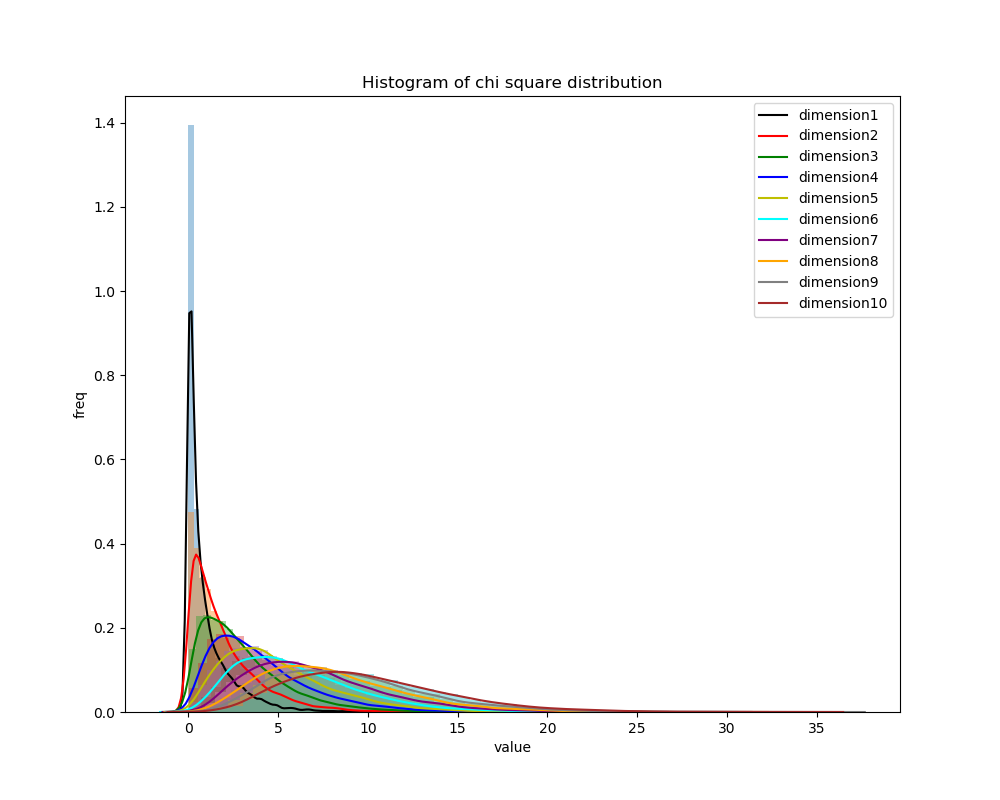
\includegraphics[clip, scale=0.6]{hist.png}
    \caption{自由度が1-10のカイ二乗分布のヒストグラム}
  \end{center}
\end{figure}
\end{document}